\documentclass[11pt]{exam}

\usepackage{amssymb, amsmath, amsthm, mathrsfs, multicol, graphicx}
\usepackage{tikz}

 \def\d{\displaystyle}
\def\?{\reflectbox{?}}
\def\b#1{\mathbf{#1}}
\def\f#1{\mathfrak #1}
\def\c#1{\mathcal #1}
\def\s#1{\mathscr #1}
\def\r#1{\mathrm{#1}}
\def\N{\mathbb N}
\def\Z{\mathbb Z}
\def\Q{\mathbb Q}
\def\R{\mathbb R}
\def\C{\mathbb C}
\def\F{\mathbb F}
\def\A{\mathbb A}
\def\X{\mathbb X}
\def\E{\mathbb E}
\def\O{\mathbb O}
\def\U{\mathcal U}
\def\pow{\mathcal P}
\def\inv{^{-1}}
\def\nrml{\triangleleft}
\def\st{:}
\def\~{\widetilde}
\def\rem{\mathcal R}
\def\sigalg{$\sigma$-algebra }
\def\Gal{\mbox{Gal}}
\def\iff{\leftrightarrow}
\def\Iff{\Leftrightarrow}
\def\land{\wedge}
\def\And{\bigwedge}
\def\AAnd{\d\bigwedge\mkern-18mu\bigwedge}
\def\Vee{\bigvee}
\def\VVee{\d\Vee\mkern-18mu\Vee}
\def\imp{\rightarrow}
\def\Imp{\Rightarrow}
\def\Fi{\Leftarrow}

%\def\={\equiv}
\def\var{\mbox{var}}
\def\mod{\mbox{Mod}}
\def\Th{\mbox{Th}}
\def\sat{\mbox{Sat}}
\def\con{\mbox{Con}}
\def\bmodels{=\joinrel\mathrel|}
\def\iffmodels{\bmodels\models}
\def\dbland{\bigwedge \!\!\bigwedge}
\def\dom{\mbox{dom}}
\def\rng{\mbox{range}}
\DeclareMathOperator{\wgt}{wgt}


\def\bar{\overline}


\newcommand{\vtx}[2]{node[fill,circle,inner sep=0pt, minimum size=4pt,label=#1:#2]{}}
\newcommand{\va}[1]{\vtx{above}{#1}}
\newcommand{\vb}[1]{\vtx{below}{#1}}
\newcommand{\vr}[1]{\vtx{right}{#1}}
\newcommand{\vl}[1]{\vtx{left}{#1}}
\renewcommand{\v}{\vtx{above}{}}

\def\circleA{(-.5,0) circle (1)}
\def\circleAlabel{(-1.5,.6) node[above]{$A$}}
\def\circleB{(.5,0) circle (1)}
\def\circleBlabel{(1.5,.6) node[above]{$B$}}
\def\circleC{(0,-1) circle (1)}
\def\circleClabel{(.5,-2) node[right]{$C$}}
\def\twosetbox{(-2,-1.4) rectangle (2,1.4)}
\def\threesetbox{(-2.5,-2.4) rectangle (2.5,1.4)}
\newcommand{\twoline}[2]{\begin{pmatrix}#1 \\ #2 \end{pmatrix}}


\def\d{\displaystyle}
\def\?{\reflectbox{?}}
\def\b#1{\mathbf{#1}}
\def\f#1{\mathfrak #1}
\def\c#1{\mathcal #1}
\def\s#1{\mathscr #1}
\def\r#1{\mathrm{#1}}
\def\N{\mathbb N}
\def\Z{\mathbb Z}
\def\Q{\mathbb Q}
\def\R{\mathbb R}
\def\C{\mathbb C}
\def\F{\mathbb F}
\def\A{\mathbb A}
\def\X{\mathbb X}
\def\E{\mathbb E}
\def\O{\mathbb O}
\def\pow{\mathscr P}
\def\inv{^{-1}}
\def\nrml{\triangleleft}
\def\st{:}
\def\~{\widetilde}
\def\rem{\mathcal R}
\def\iff{\leftrightarrow}
\def\Iff{\Leftrightarrow}
\def\and{\wedge}
\def\And{\bigwedge}
\def\AAnd{\d\bigwedge\mkern-18 mu\bigwedge}
\def\Vee{\bigvee}
\def\VVee{\d\Vee\mkern-18 mu\Vee}
\def\imp{\rightarrow}
\def\Imp{\Rightarrow}
\def\Fi{\Leftarrow}



\def\circleA{(-.5,0) circle (1)}
\def\circleAlabel{(-1.5,.6) node[above]{$A$}}
\def\circleB{(.5,0) circle (1)}
\def\circleBlabel{(1.5,.6) node[above]{$B$}}
\def\circleC{(0,-1) circle (1)}
\def\circleClabel{(.5,-2) node[right]{$C$}}
\def\twosetbox{(-2,-1.5) rectangle (2,1.5)}
\def\threesetbox{(-2,-2.5) rectangle (2,1.5)}


\def\bar{\overline}

%\pointname{pts}
\pointsinmargin
\marginpointname{pts}
\marginbonuspointname{ bns pts}

\addpoints
\pagestyle{headandfoot}
%\printanswers

\firstpageheader{Math 228}{\bf\large Exam 3 (Makeup)}{November 27, 2017}
\runningfooter{}{\thepage}{}
\extrafootheight{-.45 in}



\begin{document}
%space for name
\noindent {\large\bf Name:} \underline{\hspace{2.5 in}}
\vskip 1em

\noindent{\bf Instructions:} Answer each of the following questions.  Answers without supporting work or explanations will be counted as incorrect.  When asked to explain, justify, or prove your answers, use complete English sentences.



\begin{questions}

\question[10] Simplify:
\[\neg(P \imp Q)\]
\begin{solution}
\[P \wedge \neg Q\]
\end{solution}
\vskip 4 em

\question[18] Remember that by a \emph{degree sequence} we mean the list of degrees (from largest to smallest) of each vertex in the graph.  Consider the statement,

\begin{center}
	\textit{If $G_1$ and $G_2$ are graphs with the same degree sequence, then $G_1$ and $G_2$ are isomorphic.}
\end{center}

\begin{parts}
	\part If this were true, how would you start a proof?  Write the \underline{first line} of a proof of the statement using each specified style of proof:

	Direct proof:
	\begin{solution}
	Assume $G_1$ and $G_2$ have the same degree sequence.
	\end{solution}

	\vskip 3 em

	Proof by contrapositive:
	\begin{solution}
Assume $G_1$ and $G_2$ are NOT isomorphic.
	\end{solution}

	\vskip 3 em

	Proof by contradiction:
	\begin{solution}
	Assume $G_1$ and $G_2$ have the same degree sequence but are NOT isomorphic.
	\end{solution}
	\vskip 3 em

	\part Prove that the statement is in fact false by giving a counterexample: Let $G_1 = (V_1, E_1)$ have $V_1 = \{a,b,c,d,e,f\}$ and $E_1 = \{ab, bc, cd, ce, de, ef\}$.  Find a graph $G_2$ with the same degree sequence as $G_1$ but which is not isomorphic to $G_1$.  Explain how you know the graphs are not isomorphic.
	\begin{solution}
	One way to draw $G_1$ is

	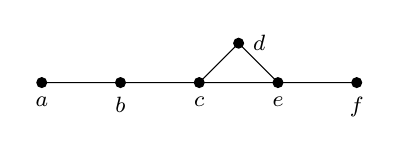
\begin{tikzpicture}
		\footnotesize{
		\draw (0,0) \vb{$a$} -- (1,0) \vb{$b$} -- (2,0) \vb{$c$} -- (3,0) \vb{$e$} -- (4,0) \vb{$f$} (2,0) -- (2.5, 0.5) \vr{$d$} -- (3,0);
		}
	\end{tikzpicture}

Let $G_2$ be the graph shown here:

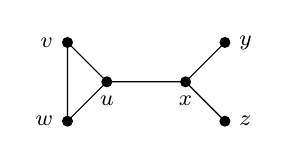
\begin{tikzpicture}
	\footnotesize{
	\draw (0,0) \vb{$u$} -- (-.5, .5) \vl{$v$} -- (-.5, -.5) \vl{$w$} -- (0,0) -- (1,0) \vb{$x$} -- (1.5, .5) \vr{$y$} (1,0) -- (1.5, -.5) \vr{$z$};
	}
\end{tikzpicture}

Both graphs have degree sequence $(3,3,2,2,1,1,)$.  However, there is not an isomorphism between $G_1$ and $G_2$.  If there were, we would need to match up vertices with the same degree.  Look at the vertices of degree 2 in each graph.  In $G_1$, these are $b$ and $d$, which are not adjacent.  In $G_2$, these are $v$ and $w$, which are adjacent.
	\end{solution}


	\vfill


\end{parts}



\newpage

\question Consider the statement: ``If a graph has chromatic number at most 4, then it is planar or has an Euler path.''
\begin{parts}
\part[12] Complete a truth table for the statement: $C \imp (P \vee E)$

\renewcommand{\arraystretch}{1.5}
  \begin{tabular}{c|c|c||c}

  $C$ & $P$ & $E$ & \hspace{5 in} \\ \hline
  T & T & T & \\
  T & T & F & \\
  T & F & T & \\
  T & F & F & \\
  F & T & T & \\
  F & T & F & \\
  F & F & T & \\
  F & F & F & \\
  \end{tabular}
\begin{solution}

\renewcommand{\arraystretch}{1.5}
  \begin{tabular}{c|c|c||c}

  $C$ & $P$ & $E$ & $C \imp (P \vee E)$ \\ \hline
  T & T & T & T\\
  T & T & F & T\\
  T & F & T & T\\
  T & F & F & F\\
  F & T & T & T\\
  F & T & F & T\\
  F & F & T & T\\
  F & F & F & T\\
  \end{tabular}
\end{solution}

\vskip 2 em

\part[8] Your friend believes the statement is false, and gives $K_5$ as a counter example.  What row in the truth table does $K_5$ correspond to?  \underline{Use the truth table} to explain $K_5$ is NOT a counterexample to the statement.
\begin{solution}
$K_5$ has chromatic number 5, so not at most 4, is not planar and has an Euler path.  This corresponds to the 7th row of the truth table.  But the statement is true in that case, so $K_5$ does not prove the statement is false.
\end{solution}

\vfill

\part[6] Prove that the statement is indeed false by giving a correct counterexample.
\begin{solution}
	We need a graph that has chromatic number at most 4, but is not planar and does not have an Euler path.  $K_{3,3}$ is such a graph.  It's bipartite so its chromatic number is 2.  We saw in class that it is not planar.  Also, since every vertex has degree 3, we know that $K_{3,3}$ does not have an Euler path.
\end{solution}

\vfill
\end{parts}

% \newpage
%
% \question[18] Suppose $G$ is a graph with 7 vertices.  Consider the statement:
% \vskip 1em
% \centerline{\textit{If $G$ has an Euler circuit, then there are at least 3 vertices with the same degree.}}
% \vskip 1em
% \begin{parts}

% \part  Prove the statement using an appropriate style of proof.  Hint: what could the degrees be?
% \begin{solution}
% \begin{proof}
% Proceed by contradiction.  Assume $G$ has an Euler circuit and that there are at most 2 vertices sharing the same degree.  Since $G$ has an Euler circuit, every vertex has \emph{even} degree.  Thus the possible degrees are 2, 4, and 6 (you cannot have larger degree since there are only 7 vertices).  Since there are at most 2 vertices sharing the same degree, there are at most 6 vertices.  This contradicts the assumption that $G$ has 7 vertices.
% \end{proof}
%
% \end{solution}
% \vfill
% \end{parts}

\newpage

\question[22] Consider the graph drawn below:

\begin{center}
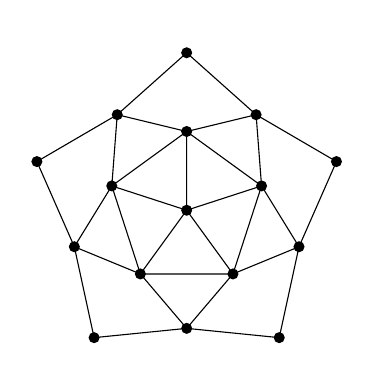
\begin{tikzpicture}

\foreach \x in {0,...,4} {
	\coordinate (a\x) at (18+\x*72:1cm);
	\coordinate (b\x) at (18+\x*72:2cm);
	\coordinate (c\x) at (54+\x*72:1.5cm);
	\draw (0,0) -- (a\x) \v -- (c\x) \v -- (b\x) \v;
}
\draw (0,0) \v;
\draw (a0) -- (a1) -- (a2) -- (a3) -- (a4) -- (a0);
\draw (a0) -- (c4) (a1) -- (c0) (a2) -- (c1) (a3) -- (c2) (a4) -- (c3);
\draw (b0) -- (c4) (b1) -- (c0) (b2) -- (c1) (b3) -- (c2) (b4)-- (c3);
\end{tikzpicture}
\end{center}

\begin{parts}
\part Find a proper vertex coloring of the graph.  Color (or label) the graph above.

\begin{solution}
	You \emph{could} color every vertex a different color.  Or you could use as few as 4 colors: start with the center vertex and use three other colors for the adjacent vertices.  Continue working your way out.
\end{solution}


\part Explain how you know the chromatic number of the graph cannot be more than 4.
\begin{solution}
The graph is planar, so the chromatic number is at most 4.  Alternatively, if you gave a 4-coloring above, you know the chromatic number must be 4 or less.
\end{solution}

\vfill
\part Explain how you know the chromatic number of the graph cannot be less than 4.
\begin{solution}
The vertex in the center and its 5 neighbors create a copy of $W_5$ (the 5-wheel), which requires 4 colors.  The cycle of 5 vertices requires 3 colors, and the center vertex must be a different color than those three.
\end{solution}
\vfill
\part Does the graph contain an Euler path?  Explain.
\begin{solution}
No.  There are more than 2 vertices with odd degree (in fact, there are 6 vertices of degree 5).  Any vertex with odd degree in an Euler path which is not the starting vertex will be a vertex we eventually get stuck at.
\end{solution}
\vfill
\end{parts}

\newpage












\question Consider (connected) graphs in which every vertex has degree 7.  Let $v$ be the number of vertices in such a graph.
\begin{parts}
  \part[6] Suppose $v = 10$.  How many \emph{edges} does the graph have.  Briefly explain.
  \begin{solution}
   54.  Each of the 12 vertices has degree 7, so the sum of the degrees is $10 \cdot 7 = 70$.  But the sum of the degrees counts each edge twice since each edge is attached to exactly two vertices.  So the number of edges is half the sum of the degrees, so 35.
  \end{solution}

  \vfill
  \part[8] Which of the following numbers of vertices are also possible?  Remember, all vertices have degree 7.  \underline{Circle} all that are possible and \underline{cross out} all that are impossible.  Briefly explain.
  \[v = 6  \hspace{1in} v = 8 \hspace{1in} v = 9 \hspace{1in} v = 103\]
  \begin{solution}
   Since this is a graph and not a multigraph, we must have $v$ at least 8 (this would give $K_{8}$).  Additionally, $v$ cannot be any odd number -- if we had an odd number of vertices, then the sum of the degrees would be odd, which is impossible, since the sum of the degrees is {\em twice} the number of edges.  Thus the only one above that is possible is $v = 8$.
  \end{solution}

  \vfill
  \part[10] Again, let $v = 10$.  Prove that the graph is NOT planar.    Your proof should be written out in words and it should be clear what style of proof you are using.
  \begin{solution}
   We have seen that the graph has 10 vertices and 35 edges.  Now if the graph were planar, it would satisfy Euler's formula, $v - e + f = 2$, which would say that there must be 27 faces.  However, since the graph is not a multigraph, each face would be bounded by at least 3 edges, with each edge part of the boundary for two faces.  So we would have
   \[3f \le 2e\]
   But we have 27 faces and 35 edges, which would say that $81 \le 70$, a contradiction.  Therefore the graph is not planar.
  \end{solution}

  \vfill
  \vfill

\end{parts}


\newpage

\bonusquestion[10] Bonus!! Before you sit three chests -- one made of wood, one of stone, and one of steel.  You know that one of the chests contains a great treasure, while the other two contain vicious, angry, man-eating, deadly poisonous scorpions (also known as {\em scorpions}).

On each chest hangs a sign, giving you information about which chest contains the treasure.  Problem is, you do not know which signs are true and which are false.  The signs read:
\begin{itemize}
  \item[Wood chest:] If the sign on the stone chest is true, then the treasure is not in the steel chest.
  \item[Stone chest:] Exactly two of these signs are false. % and the treasure is not in this chest.
  \item[Steel chest:] The treasure is in a chest with a false sign.
\end{itemize}
Which chest contains the treasure?  Prove your answer is correct.

(For some partial credit, determine the truth or falsity of one or more signs and explain.)

\begin{solution}
 The treasure is in the stone chest.

 \begin{proof}
  Consider the stone chest's sign.  If the sign were true, then both of the other signs would be false.  However, the wood chest's sign being false means that the sign on the stone chest is true {\em and} the treasure {\em is} in the steel chest.  So the treasure would be in the steel chest, a chest with a false sign, making the steel chest's sign true.  This is a contradiction.  Therefore the stone chest's sign must be false.

  Now we know that either all three signs are false or just the stone chest's sign is false (if one other sign was false, that would be two false signs, which we know is not the case).  However, it cannot be that all three signs are false: if the wood chest's sign is false, that means the stone chest's sign is true, a possibility we have already discounted.  Therefore the signs on both the wood and steel chests are true.  In particular, it is true that the treasure is in a chest with a false sign.  There is only one such chest: the stone chest, wherein lies the treasure.
 \end{proof}

\end{solution}



%\question[16] Consider the graph below.
%\begin{center}
%\begin{tikzpicture}
%\coordinate (a) at (-.25,3);
%\coordinate (b) at (1,4);
%\coordinate (c) at (2.25,3);
%\coordinate (d) at (1,1.25);
%\coordinate (e) at (3,1.5);
%\coordinate (f) at (2.75,.5);
%\coordinate (g) at (1,0);
%\coordinate (h) at (.25, .5);
%\coordinate (i) at (-1,-.25);
%
%\draw (a) \vtx{above left}{$a$} -- (b) \vtx{above}{$b$} -- (c) \vtx{above right}{$c$} -- (d) \vtx{above}{$d$} -- (e) \vtx{above right}{$e$} -- (f) \vtx{right}{$f$} -- (g) \vtx{below}{$g$} -- (h) \vtx{above left}{$h$} (g) -- (i) \vtx{left}{$i$} -- (a) -- (c) -- (e) -- (d) -- (f) (d) -- (g) (d) -- (h) (d) -- (a);
%
%\end{tikzpicture}
%\end{center}
%
%%\begin{figure}[h]
%%\begin{center}
%%\includegraphics[height=1.8 in, width=1.8 in]{ExamEulerPath}
%%\end{center}
%%\end{figure}
%
%\begin{parts}
%\part Is there an Euler path that starts at vertex $a$? If so, describe the path.  If not, say specifically what goes wrong.
%\begin{solution}
%No there is not.  The graph has two vertices with odd degree ($e$ and $f$), so any Euler path would have to start at one of those vertices.  If we started at $a$, we would get stuck at either $e$ or $f$ because we would go to the vertex, leave it again, then go to it a third time, and not be able to leave.  We can stop at a vertex other than $a$, but if we stop at $e$, we won't be able to use all 3 edges incident to $f$ (or visa-versa).
%\end{solution}
%\vfill
%\part Is there an Euler path that starts at a different vertex? Explain.
%\begin{solution}
%Yes, we could start at either $e$ or $f$ (and end at the other one).  All the other vertices have even degree, so we can go to, and leave, them an equal number of times.  One such path is:
%\[e,c,b,a,i,g,f,d,g,h,d,a,c,d,e,f\]
%\end{solution}
%\vfill
%\end{parts}
%\newpage



%\question[16] Use a truth table to decide whether the following argument form is valid:

%\begin{center}
%\begin{tabular}{rl} & $(P \vee Q) \imp R$ \\ & $P \and \neg R$ \\ \hline $\therefore$ & $Q \imp R$\end{tabular}
%\end{center}

%\begin{center}
%  \begin{tabular}{c|c|c||c}
%
%  $B$ & $E$ & $P$ & \hspace{5in} \\ \hline & & & \\
%  T & T & T & \\ & & & \\
%  T & T & F & \\ & & & \\
%  T & F & T & \\ & & & \\
%  T & F & F & \\ & & & \\
%  F & T & T & \\ & & & \\
%  F & T & F & \\ & & & \\
%  F & F & T & \\ & & & \\
%  F & F & F & \\
%  \end{tabular}

%\end{center}
%\begin{solution}
% \begin{center}
%  \begin{tabular}{c|c|c||c|c|c}
%
%  $P$ & $Q$ & $R$ & $(P \vee Q) \imp R$ & $P \and \neg R$ & $Q \imp R$ \\ \hline & & & & & \\
%  T & T & T & T & F & T \\ & & & & & \\
%  T & T & F & F & T & F \\ & & & & & \\
%  T & F & T & T & F & T\\ & & & & & \\
%  T & F & F & F & T & T\\ & & & & & \\
%  F & T & T & T & F & T \\ & & & & & \\
%  F & T & F & F & F & F\\ & & & & & \\
%  F & F & T & T & F & T\\ & & & & & \\
%  F & F & F & T & F & T
%  \end{tabular}
%
%\end{center}
%\end{solution}
%
%The argument is: Valid / Not Valid (circle one).
%
%Explain:
%\begin{solution}
% The argument is \underline{valid}.  An argument is valid provided whenever all the premises are true, the conclusion must be true.  So an argument is not valid if there is any possibility of all premises being true and the conclusion being false.
%
% In this example, there is no way for both premises to be true.  Therefore, there is no way for the premises to be true and the conclusion false, so the argument is not invalid - it is therefore valid.
%\end{solution}


%%FIX:
%\question[18] Consider the statement: \[\forall f (\exists x \exists y (f(x) < 0 \and f(y) > 0) \imp \exists z (f(z) = 0) ).\]  For each task below, show your steps to clearly illustrate how you arrive at your final answer.
%\begin{parts}
% \part Write the converse of the statement (in symbols), simplifying as much as possible.
% \begin{solution}
%  $\forall f (\exists z (f(z) = 0) \imp \exists x \exists y (f(x) < 0 \and f(y) > 0))$
% \end{solution}
%
% \vfill
% \part Write the contrapositive of the statement (in symbols), simplifying as much as possible.
% \begin{solution}
%  $\forall f (\forall z (f(z) \ne 0) \imp \forall x \forall y (f(x) \ge 0 \vee f(y) \le 0))$
% \end{solution}
%
% \vfill
% \part Write the negation of the statement (in symbols), simplifying as much as possible.
% \begin{solution}
%  $\exists f ( \exists x \exists y(f(x) < 0 \and f(y) > 0) \and \forall z (f(z) \ne 0))$.
% \end{solution}
%
% \vfill
%\end{parts}
%
%
%
%\newpage


%\newpage
%
%\question[12] Consider the following graph:
%\vspace{-1em}
%\begin{center}
% \begin{tikzpicture}[scale=.7]
%  \draw[thick] (-2,-1) \v -- (-2,1) \v -- (-.5,.5) \v -- (.5, .5) \v -- (2, 1) \v -- (2, -1) \v -- (.5, -.5) \v -- (-.5, -.5) \v -- (-2, -1) (-.5, .5) -- (.5, -.5) -- (.5, .5) -- (-.5, -.5) -- (-.5, .5);
% \end{tikzpicture}
%\end{center}
%
%\begin{parts}
% \part Is the graph planar?  Briefly explain.
%\begin{solution}
%  Yes.  It is possible to draw the graph so that no edges cross.  For example:
%  \begin{center}
% \begin{tikzpicture}[scale=.7]
%  \draw[thick] (-2,-1) \v -- (-2,1) \v -- (-.5,.5) \v -- (.5, .5) \v -- (2, 1) \v -- (2, -1) \v -- (.5, -.5) \v -- (-.5, -.5) \v -- (-2, -1) (-.5, .5) to[out=45, in=180] (2,2) to[out=0, in=90] (3,0) to[out=270,in=0] (2,-2) to[out=180,in=-90] (.5, -.5) -- (.5, .5) -- (-.5, -.5) -- (-.5, .5);
% \end{tikzpicture}
%\end{center}
%\end{solution}
%
% \vfill
% \part What is the chromatic number of the graph?  Briefly explain.
%
% \begin{solution}
%  4.  The center four vertices are all adjacent to each other - they form a $K_4$ subgraph.  No matter what, you will need 4 colors for these vertices.  The outside vertices can repeat these colors easily.  In fact, we know that since the graph is planar, we won't need to use more than 4 colors by the four color theorem.
% \end{solution}
%
% \vfill
% \part Does the graph have an Euler circuit?  Briefly explain.
% \begin{solution}
%  Yes.  Every vertex has even degree, so there is an Euler circuit.
% \end{solution}
%
% \vfill
%\end{parts}

% LAST TIME:
%
% \question[8] Complete the truth table below for the statement $P \and \neg(Q \imp R)$.
%
% \vskip 1em
%
% \begin{center}
%   \begin{tabular}{c|c|c||c}
%
%   $P$ & $Q$ & $R$ & \hspace{5in} \\ \hline & & & \\
%   T & T & T & \\ & & & \\
%   T & T & F & \\ & & & \\
%   T & F & T & \\ & & & \\
%   T & F & F & \\ & & & \\
%   F & T & T & \\ & & & \\
%   F & T & F & \\ & & & \\
%   F & F & T & \\ & & & \\
%   F & F & F & \\
%   \end{tabular}
%
% \end{center}
%
% \question[4] If the statement $P \and \neg(Q \imp R)$ is true, what can you conclude about $P$, $Q$, and $R$? Explain.
% \vfill
% \question[8] Draw (shade in) a Venn diagram for the set $A \cap \bar{(\bar B \cup C)}$
% \vfill
%
% \newpage
% \question[20] Consider the statement, ``for all integers $a$ and $b$, if $a + b$ is odd, then $a$ or $b$ is odd.''
% \begin{parts}
%   \part How would a {\em direct} proof of the statement begin and end?
%   \vskip 1ex
%   First two lines:
%   \vfill
%   Last line:
%   \vskip 3em
%   \part How would a {\em proof by contrapositive} of the statement begin and end?
%   \vskip 1ex
%   First two lines:
%   \vfill
%   Last line:
%   \vskip 3em
%   \part How would a {\em proof by contradiction} of the statement begin and end?
%   \vskip 1ex
%   First line:
%   \vfill
%   Last line:
%   \vskip 3em
%   \part Prove the statement by the appropriate proof method.
%   \vfill
%   \vfill
%   \vfill
% \end{parts}
%
%
% \newpage
%
% \question[12] Find the converse, contrapositive, and negation of the statement:
% \begin{center}
%   For all integers $n$, if $n$ is even and prime, then $n = 2$.
% \end{center}
% \begin{parts}
%   \part Converse:
%   \vfill
%   \part Contrapositive:
%   \vfill
%   \part Negation:
%   \vfill
% \end{parts}
%
%
% \question[8] Consider the set $A = \{2, 3, 7, \{2,3,4\}, \{\emptyset\}, \heartsuit\}$
% \begin{parts}
%   \part Find $|A|$.
%   \vfill
%   \part Give an example of a set $B$ for which $B \subset A$.
%   \vfill
%   \part Give an example of a set $B$ for which $B \in A$.
%   \vfill
%   \part Are there any sets $B$ for which $B \subset A$ and $B \in A$?  Find one or explain why not.
%   \vfill
% \end{parts}
%
%
%
% \newpage
%
% \question[10] Explain, using a Venn diagram, why $|A \cup B| = |A| + |B| - |A \cap B|$.
% \vfill
%
%
% \question[12] Consider the function $f:\N \to \N$ (where $\N$ is the set of natural numbers) defined by
% \[f(n) = \begin{cases}
%            n+4 & \mbox{ if $n$ is even}\\
%            2n & \mbox{ if $n$ is odd}
%          \end{cases}\]
% \begin{parts}
%   \part Is $f$ an injection (i.e., one-to-one)?  Explain.
%   \vfill
%   \part Is $f$ a surjection (i.e., onto)?  Explain.
%   \vfill
% \end{parts}
%
%
%
% \newpage
% \question[6] Simplify the following statements:
% \begin{parts}
%  \part $\neg(\neg S \and (P \imp (\neg Q \vee R)))$
%  \vfill
%  \part $\neg \exists x \forall y (x < y \vee \forall z (x = y + z))$
%  \vfill
% \end{parts}
%
%
% \question[12] Let $f:\N \to \N$ be a function.
% \begin{parts}
%   \part Is it possible for $f\inv(5) = \{1,2\}$ and $f\inv(6) = \{2,3\}$?  Explain why or why not.
%   \vfill
%   \vfill
%   \part Could it be that $f\inv(1) = \{4,5,9\}$?  If so, what does this tell you about the function $f$?  Explain.
%   \vfill
%   \vfill
%   \part Could it be that $f\inv(2) = \emptyset$?  If so, what does this tell you about the function $f$?  Explain.
%   \vfill
%   \vfill
% \end{parts}
%
% \newpage
%
% \bonusquestion[10] Bonus!  Suppose you know the following information about the sets $A$, $B$ and $C$:
% \[|A| = 30 \qquad |B| = 26 \qquad |C| = 28\]
% \[|A \cap B| = 18 \qquad |A \cap C| = 20 \qquad |B \cap C| = 15\]
% \[|A \cap B \cap C| = 10\]
% Find a set $S$, expressed in terms of $A$, $B$, and $C$ such that $|S| = 34$.  Show your work.
%
% (For full credit, your set $S$ should be simplified as much as possible.)

\end{questions}




\end{document}
